\RequirePackage{currfile}
\documentclass[12pt]{beamer}
\usepackage[utf8]{inputenc}
\usepackage[spanish]{babel}
\usepackage{standalone}
\usepackage{color}
\usepackage{siunitx}
\usepackage{hyperref}
%\hypersetup{colorlinks,linkcolor=,urlcolor=blue}
%\hypersetup{colorlinks,urlcolor=blue}
\usepackage{xcolor,soul}
\usepackage{etoolbox}
\usepackage{amsmath}
\usepackage{amsthm}
\usepackage{physics}
\usepackage{multicol}
\usepackage{bookmark}
\usepackage{longtable}
\usepackage{listings}
\usepackage{graphicx}
\usepackage{tikz}
\usetikzlibrary{patterns, matrix, backgrounds, decorations,shapes, arrows.meta}
\usepackage[autostyle,spanish=mexican]{csquotes}
\usepackage[os=win]{menukeys}
\usepackage{pifont}
\usepackage{pbox}
\usepackage{caption}
\captionsetup{font=scriptsize,labelfont=scriptsize}
%\usepackage[sfdefault]{roboto}  %% Option 'sfdefault' only if the base font of the document is to be sans serif

%Sección de definición de colores
\definecolor{ao}{rgb}{0.0, 0.5, 0.0}
\definecolor{bisque}{rgb}{1.0, 0.89, 0.77}
\definecolor{amber}{rgb}{1.0, 0.75, 0.0}
\definecolor{armygreen}{rgb}{0.29, 0.33, 0.13}
\definecolor{alizarin}{rgb}{0.82, 0.1, 0.26}
\definecolor{cadetblue}{rgb}{0.37, 0.62, 0.63}
\definecolor{deepblue}{rgb}{0,0,0.5}
\definecolor{brown}{rgb}{0.59, 0.29, 0.0}
\definecolor{OliveGreen}{rgb}{0,0.25,0}


\usefonttheme[onlymath]{serif}
%Sección de definición de nuevos comandos

\newcommand*{\TitleParbox}[1]{\parbox[c]{1.75cm}{\raggedright #1}}%
\newcommand{\python}{\texttt{python}}
\newcommand{\textoazul}[1]{\textcolor{blue}{#1}}
\newcommand{\azulfuerte}[1]{\textcolor{blue}{\textbf{#1}}}
\newcommand{\funcionazul}[1]{\textcolor{blue}{\textbf{\texttt{#1}}}}
\newcommand{\ptilde}[1]{\ensuremath{{#1}^{\prime}}}
\newcommand{\stilde}[1]{\ensuremath{{#1}^{\prime \prime}}}
\newcommand{\ttilde}[1]{\ensuremath{{#1}^{\prime \prime \prime}}}
\newcommand{\ntilde}[2]{\ensuremath{{#1}^{(#2)}}}
\renewcommand{\arraystretch}{1.5}

\newcounter{saveenumi}
\newcommand{\seti}{\setcounter{saveenumi}{\value{enumi}}}
\newcommand{\conti}{\setcounter{enumi}{\value{saveenumi}}}
\renewcommand{\rmdefault}{cmr}% cmr = Computer Modern Roman

\linespread{1.5}

\usefonttheme{professionalfonts}
%\usefonttheme{serif}
\DeclareGraphicsExtensions{.pdf,.png,.jpg}


%Sección para el tema de beamer, con el theme, usercolortheme y sección de footers
\mode<presentation>
{
  \usetheme{Warsaw}
  
  %\useoutertheme{infolines}
  \useoutertheme{default}
  \usecolortheme{spruce}
  \setbeamercovered{invisible}
  % or whatever (possibly just delete it)
  \setbeamertemplate{section in toc}[sections numbered]
  \setbeamertemplate{subsection in toc}[subsections numbered]
  \setbeamertemplate{subsection in toc}{\leavevmode\leftskip=3.2em\rlap{\hskip-2em\inserttocsectionnumber.\inserttocsubsectionnumber}\inserttocsubsection\par}
  \setbeamercolor{section in toc}{fg=blue}
  \setbeamercolor{subsection in toc}{fg=blue}
  \setbeamercolor{frametitle}{fg=blue}
  \setbeamertemplate{caption}[numbered]

  \setbeamertemplate{footline}
  \beamertemplatenavigationsymbolsempty
  \setbeamertemplate{headline}{}
}

\makeatletter
\setbeamercolor{section in foot}{bg=gray!30, fg=black!90!orange}
\setbeamercolor{subsection in foot}{bg=blue!30!yellow, fg=red}
\setbeamertemplate{footline}
{
  \leavevmode%
  \hbox{%
  \begin{beamercolorbox}[wd=.333333\paperwidth,ht=2.25ex,dp=1ex,center]{section in foot}%
    \usebeamerfont{section in foot} \insertsection
  \end{beamercolorbox}}%
  \begin{beamercolorbox}[wd=.333333\paperwidth,ht=2.25ex,dp=1ex,center]{subsection in foot}%
    \usebeamerfont{subsection in foot}  \insertsubsection
  \end{beamercolorbox}%
  \begin{beamercolorbox}[wd=.333333\paperwidth,ht=2.25ex,dp=1ex,right]{date in head/foot}%
    \usebeamerfont{date in head/foot} \insertshortdate{} \hspace*{2em}
    \insertframenumber{} / \inserttotalframenumber \hspace*{2ex} 
  \end{beamercolorbox}}%
  \vskip0pt%
\makeatother  

\makeatletter
\patchcmd{\beamer@sectionintoc}
  {\vfill}
  {\vskip\itemsep}
  {}
  {}
\makeatother


\title{\large{Asesorías}}
\author{M. en C. Gustavo Contreras Mayén}
\date{\today}
\institute{Facultad de Ciencias - UNAM}
\titlegraphic{
\includegraphics[width=1.75cm]{../Imagenes/escudo-facultad-ciencias}\hspace*{4.75cm}~%
   
\includegraphics[width=1.75cm]{../Imagenes/escudo-unam}
}
\setbeamertemplate{navigation symbols}{}
\begin{document}
\maketitle
\fontsize{14}{14}\selectfont
\spanishdecimal{.}
\section*{Contenido}
\frame{\tableofcontents[currentsection, hideallsubsections]}

\begin{frame}
\frametitle{Dinámica de la sesión}
Les pedimos amablemente que conforme vaya avanzando la exposición, si tienen alguna duda o comentario, lo vayan anotando en el chat.
\\
\bigskip
\pause
Nuestra intención es responder cada una de las preguntas o comentarios para contar con las respuestas.
\end{frame}

\section{Objetivos}
\frame{\tableofcontents[currentsection, hideothersubsections]}
\subsection{Objetivo general}

\begin{frame}
\frametitle{Objetivo de las asesorías}
El objetivo de las asesorías es generar una reactivación paulatina en el ritmo de trabajo que se había establecido al iniciar el semestre.
\end{frame}
\begin{frame}
\frametitle{Objetivo de las asesorías}
La inercia establecida tanto por la contingencia como por el paro, ha provocado una inercia e incertidumbre sobre la continuidad en las actividades académicas.
\end{frame}
\begin{frame}
\frametitle{Beneficios en las asesorías}
El retomar el trabajo brindará un cambio positivo para que en el momento de tener al aviso oficial de continuar el semestre, esperamos que el regreso sea lo más accesible, amigable y con un ánimo para el trabajo académico.
\end{frame}

\section{Aclaraciones importantes}
\frame{\tableofcontents[currentsection, hideothersubsections]}
\subsection{¿Qué son las asesorías?}

\begin{frame}
\frametitle{¿Qué son las asesorías?}
Las asesorías son reuniones de participación voluntaria en donde se realizarán sesiones a modo de charlas o de pláticas, para discutir mediante una exposición con ejemplos, puntos del temario del curso de MAF.
\end{frame}
\begin{frame}
\frametitle{¿Qué no son las asesorías?}
Las asesorías no son clases.
\\
\bigskip
\pause
Recordemos que las autoridades de la Facultad pidieron respetar el paro, por lo que las asesorías serán precisamente reuniones pero no son clases formales del curso.
\end{frame}
\begin{frame}
\frametitle{Participación en las asesorías}
La asistencia y participación en las asesorías es voluntaria.
\\
\bigskip
\pause
Quien decida asistir será bienvenida(o), 
\end{frame}
\begin{frame}
\frametitle{¿Y si no asisto a las asesorías?}
En caso de que la decisión personal sea la de no asistir a las videoconferencias, no hay problema alguno.
\\
\bigskip
\pause
Como se tendrá una participación voluntaria, y como no es una clase formal, no habrá ningún tipo de sanción o penalización.
\end{frame}
\begin{frame}
\frametitle{¿Entonces para qué las asesorías?}
El asistir a las asesorías nos permitirá una reactivación general para encarrilarnos en lo que se determina el regreso al semestre.
\\
\bigskip
\pause
Es como tener un entrenamiento adicional para el ejercicio.
\end{frame}
\begin{frame}
\frametitle{¿Qué va a pasar cuando termine el paro?}
Una vez que se tenga el aviso del regreso al semestre:
\setbeamercolor{item projected}{bg=blue!70!black,fg=yellow}
\setbeamertemplate{enumerate items}[circle]
\begin{enumerate}[<+->]
\item Retomaremos el curso en donde lo dejamos.
\item Se retomarán las tareas y exámenes de manera normal.
\item La evaluación ya se determinará en su momento, considerando el tiempo que se tenga para concluir el semestre.
\end{enumerate}
\end{frame}
\begin{frame}
\frametitle{¿Se va a evaluar el trabajo en las asesorías?}
Habrá algunos ejercicios a resolver con la finalidad de que apliquen lo visto en las sesiones.
\\
\bigskip
\pause
Estos ejercicios se revisarán, se comentarán por parte del equipo académico, pero NO contarán como parte de la calificación del tema o del curso.
\end{frame}
\begin{frame}
\frametitle{Si no van a evaluarse, ¿para qué tomar las asesorías?}
Como ya se mencionó, al regresar oficialmente al curso, se retomará en el punto donde se dejó, por lo que el avance continuará de acuerdo al syllabus del curso.
\\
\bigskip
\pause
Entonces cada ejercicio a cuenta, ejercicio adicional y examen-tarea, serán parte de la evaluación.
\end{frame}
\begin{frame}
\frametitle{Ventaja de las asesorías}
Entonces ya tendrán una ventaja para resolver los ejercicios que si van a contar, de tal manera que su evaluación sea favorable en función de los ejercicios que hayan revisado y resuelto.
\end{frame}
\begin{frame}
\frametitle{Si no asistes a las asesorías}
Una vez que se haya reestablecido el semestre, y que permanezcas inscrito dentro del curso, pero que no hayas participado en las asesorías, los temas del curso se revisarán conforme a lo establecido al temario.
\end{frame}
\begin{frame}
\frametitle{Si no asistes a las asesorías}
Debiendo entregar los ejercicios a cuenta, los adicionales y las tareas-examen, que serán los que determinen la evaluación del curso, esto aplica para todos las alumnas y alumnos inscritos en la asignatura de MAF.
\end{frame}
\begin{frame}
\frametitle{Participación del grupo}
Nos interesa conocer los puntos de vista de las alumnas y alumnos del grupo, es por ello que se invitó a responder la encuesta, para involucrarlos en esta planeación de las asesorías.
\end{frame}
\section{Encuesta de participación}
\frame{\tableofcontents[currentsection, hideothersubsections]}
\subsection{Resultados}
\begin{frame}
\frametitle{Resultados preliminares}
Hasta el viernes 11 de junio se tienen los siguientes resultados de la encuesta:
\\
\bigskip
\pause
Participaciones: 
\begin{align*}
23/56 \hspace{0.3cm} \Rightarrow \hspace{0.3cm} 41 \% 
\end{align*}
\end{frame}
\begin{frame}
\frametitle{Tipo de inscripción}
\begin{figure}
    \centering
    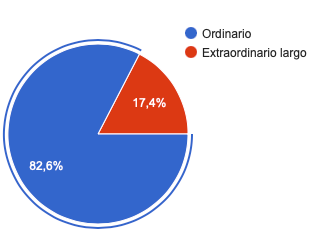
\includegraphics[scale=0.6]{Imagenes/Encuesta_Asesorias_01.png}
\end{figure}
\end{frame}
\begin{frame}
\frametitle{¿Darías de baja la asignatura?}
\begin{figure}
    \centering
    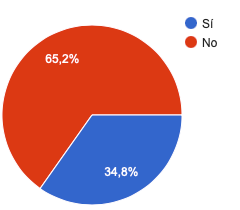
\includegraphics[scale=0.6]{Imagenes/Encuesta_Asesorias_02.png}
\end{figure}
\end{frame}
\begin{frame}
\frametitle{Participación en las asesorías}
\begin{figure}
    \centering
    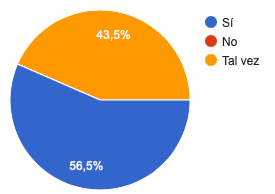
\includegraphics[scale=0.6]{Imagenes/Encuesta_Asesorias_03.png}
\end{figure}
\end{frame}
\begin{frame}
\frametitle{Participación en las asesorías}
\begin{figure}
    \hspace*{-0.4cm}
    \centering
    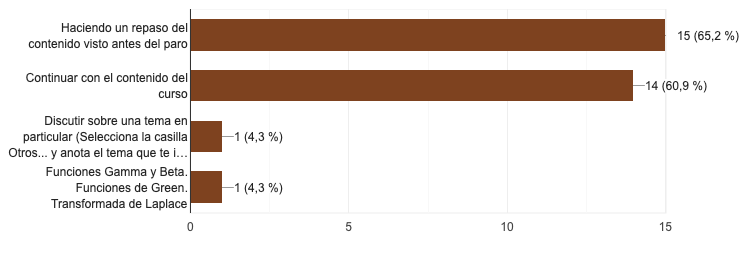
\includegraphics[scale=0.45]{Imagenes/Encuesta_Asesorias_04.png}
\end{figure}
\end{frame}
\begin{frame}
\frametitle{Evaluación del semestre}
\begin{figure}
    \centering
    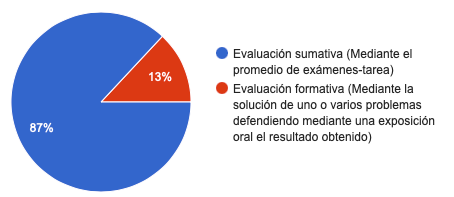
\includegraphics[scale=0.6]{Imagenes/Encuesta_Asesorias_05.png}
\end{figure}
\end{frame}

\section{Dinámica de las asesorías}
\frame{\tableofcontents[currentsection, hideothersubsections]}
\subsection{Programación}

\begin{frame}
\frametitle{Días de la semana}
Se tendrán las asesorías los días lunes y jueves en el horario correspondiente, es decir de las 3 pm a 4 pm.
\\
\bigskip
\pause
Las sesiones se realizarán mediante la plataforma Zoom.
\end{frame}
\begin{frame}
\frametitle{Materiales de trabajo}
Los materiales que ocupemos se distribuirán vía correo electrónico para quienes asistan a las sesiones de asesoría, y para aquellos que lo soliciten expresamente aunque no estén en las sesiones.
\end{frame}
\begin{frame}
\frametitle{Comunicación}
Se mantendrá una comunicación vía correo electrónico o por Telegram con el equipo académico, para atender dudas, comentarios, sugerencias, etc.
\\
\bigskip
\pause
No podremos utilizar la plataforma Moodle de la Facultad, ya que como tendremos pláticas, que no son clases formales, por lo tanto no podrán incluirse dentro del sitio oficial del curso.
\end{frame}
\begin{frame}
\frametitle{Ejercicios}
Con la finalidad de repasar lo visto en las sesiones, se dejarán uno o dos ejercicios para practicar lo revisado, teniendo la oportunidad de enviarlos para hacerles comentarios y observaciones.
\end{frame}
\begin{frame}
\frametitle{¿Qué se verá en las sesiones?}
Conforme a lo que nos expresaron en la encuesta, la propuesta de contenido es la siguiente:
\setbeamercolor{item projected}{bg=blue!70!black,fg=yellow}
\setbeamertemplate{enumerate items}[circle]
\begin{enumerate}[<+->]
\item Repaso del Tema 1.
\item Técnicas de solución: Separación de variables, remoción de singularidades y método de Frobenius.
\item Funciones especiales.
\item Transformadas integrales.
\end{enumerate}
\end{frame}
\begin{frame}
\frametitle{Alcance de los temas}
A diferencia de una clase normal, en las asesorías nos enfocaremos a presentar ejercicios y desarrollar su solución conforme al tema.
\\
\bigskip
\pause
En una clase ordinaria, se presenta el antecedente, la formalización matemática y luego los ejercicios para apoyar lo expuesto.
\end{frame}
\begin{frame}
\frametitle{Alcance de los temas}
Los temas mencionados consideramos que son los relevantes para cubrir en la asignatura.
\\
\bigskip
\pause
Ya con el semestre formal en marcha, se cubrirán otros contenidos y entonces al tocar los temas vistos en las asesorías, tendrán un repaso para entonces resolver lo que se va a evaluar.
\end{frame}
\begin{frame}
\frametitle{Evaluación del semestre}
La evaluación del semestre es un tema que se discutirá cuando ya se tenga el aviso oficial de continuar.
\\
\bigskip
\pause
No podemos adelantarnos, ya que la situación sigue siendo de incertidumbre sobre el semestre, pero tan pronto se determine el regreso, se tendrá una plática con las alumnas y alumnos que permanezcan inscritos.
\end{frame}
\begin{frame}
\frametitle{Dudas, comentarios, observaciones}
Les pedimos gentilmente que si tienen alguna duda, comentario, sugerencia, se sientan con la completa libertad de expresarlo.
\end{frame}
\end{document}

